% sections/5_1_importance_sampling_diffuse_brdf.tex
\begin{enumerate}
  \item    
    The PDF of a uniformly sampled disk of radius 1 and centered at the origin is $\frac{1}{\pi}$ when calculated using cartesian coordinates. If calculated using polar coordinates, it must be taken into account the change from $dxdy = r * d\theta dr$. This results in the PDF in polar coordinates being $\frac{r}{\pi}$.
  
  \item
    To generate samples according to the PDF using inversion sampling, we must convert the samples from a uniform distribution into samples from our unit disk. This is achieved by inverting the CDF and using marginal distributions.
    
    First we must compute the marginal distribution from either $r$ or $\theta$. In our case, we compute the marginal probability distribution with respect to $\theta$:
    
    \[p_{\theta}(\theta)=\int_{0}^{1}\frac{r}{\pi}\space dr = \left[\frac{r^{2}}{2}*\frac{1}{\pi} \right]^{1}_{0} =\frac{1}{2\pi}\]
    
    Now we must compute the CDF by taking the integral from $-\infty$ to $\theta$. Since $\theta$ is in the domain $[0,2\pi)$, we take the integral from $0$ to $\theta$.
    
    \[P_{\theta}(\theta)=\int_{0}^{\theta}\frac{1}{2\pi}\space d\theta = \left[\frac{\theta}{2\pi} \right]^{\theta}_{0} =\frac{\theta}{2\pi}\]

    We now do a similar process with $r$ conditioned to $\theta$:

    \[p(r\mid \theta)=\frac{p(r,\theta)}{p(\theta)}=\frac{\frac{r}{\pi}}{\frac{1}{2\pi}}=2r\]
    
    \[P_{r\mid \theta}(r\mid \theta)=\int_{0}^{r}2r\space dr = \left[\frac{2r^{2}}{2} \right]^{r}_{0} =r^{2}\]
    
    Now, drawing $u_{1}, u_{2}$ from a uniform distribution $U$, we need to convert them to our disk using the inverse from our CDF's:

    \[u_{1}=P_{\theta}(\theta)=\frac{\theta}{2\pi}\space; \space \theta=2\pi*u_{1}\]
    \[u_{2}=P_{{r}\mid{\theta}}(r)=r^{2}\space; \space r=\sqrt{u_{2}}\]
    Finally, we need to re-transform our polar coordinates to cartesian ones, and substitute the polar values into our uniform samples. We know the relation is:
    \[x=r\cos(\theta)=\sqrt{u_{2}}\cos(2\pi*u_{1})\] \[y=r\sin(\theta)=\sqrt{u_{2}}\sin(2\pi*u_{1})\]
  \item Code for squareToUniformDisk(Pdf)
    \begin{lstlisting}[language=C++]
Point2f Warp::squareToUniformDisk(const Point2f &sample) {
    return {
        sqrt(sample.x()) * cos(M_PI * 2 * sample.y()),
        sqrt(sample.x()) * sin(M_PI * 2 * sample.y())
    };
}

float Warp::squareToUniformDiskPdf(const Point2f &p) {
    return (p.y() * p.y() + p.x() * p.x()) <= 1 ? 1 / M_PI : 0.0f;
}
\end{lstlisting}
  \item Code for squareToCosineHemisphere(Pdf)
\begin{lstlisting}[language=C++]
  Vector3f Warp::squareToCosineHemisphere(const Point2f &sample) {
    auto disk = Warp::squareToUniformDisk(sample);
    return {
        disk.x(),
        disk.y(),
        std::sqrt(1.0f - sample.x())
    };
}

float Warp::squareToCosineHemispherePdf(const Vector3f &v) {
    if (v.z() < 0.0f) {
        return 0.0f;
    }

    // v.z() = cos(theta_i)
    return v.z() * INV_PI;
}
\end{lstlisting}

\begin{figure}[H]
    \centering
    \begin{minipage}{0.48\textwidth}
        \centering
        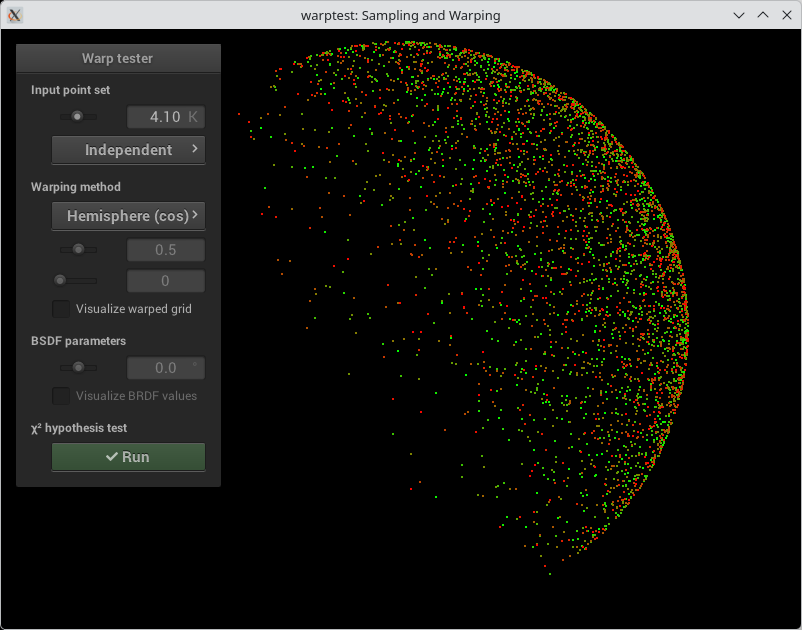
\includegraphics[width=\linewidth]{pictures/warptest-2.png}
        \caption{Transformation of independent samples into the cosine-weighted hemisphere}
        \label{fig:warp-transformation}
    \end{minipage}
    \hfill
    \begin{minipage}{0.48\textwidth}
        \centering
        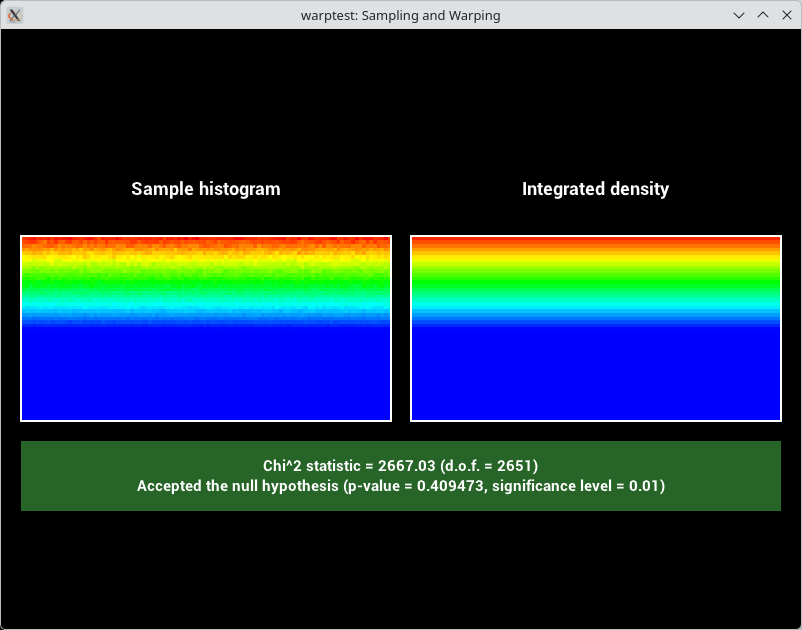
\includegraphics[width=\linewidth]{pictures/warptest-3.png}
        \caption{Successful $X^{2}$ hypothesis test}
        \label{fig:chi-square-test}
    \end{minipage}
\end{figure}
\end{enumerate}
